% ------------------------------------------------------------------------------
% TYPO3 CMS 6.2 LTS - What's New - Chapter "Install Tool" (Russian Version)
%
% @author	Andrey Aksenov <aksenovaa@bk.ru>
% @license	Creative Commons BY-NC-SA 3.0
% @link		http://typo3.org/download/release-notes/whats-new/
% @language	Russian
% ------------------------------------------------------------------------------
% Chapter: Install Tool
% ------------------------------------------------------------------------------

\section{Install Tool}
\begin{frame}[fragile]
	\frametitle{Install Tool}

	\begin{center}\huge{Глава 1:}\end{center}
	\begin{center}\huge{\color{typo3darkgrey}\textbf{Install Tool}}\end{center}

\end{frame}

% ------------------------------------------------------------------------------
% Installation
% ------------------------------------------------------------------------------

\begin{frame}[fragile]
	\frametitle{Install Tool}
	\framesubtitle{Установка}

	\begin{itemize}
		\item Теперь только \underline{единственный} пакет для установки:\newline
				\texttt{typo3\_src-6.2.x.tar.gz} (размер около 20МБ)
		\item Пакеты «Dummy» и «Blank» ушли в прошлое
		\item Установка:
			\begin{itemize}
				\item Извлеките содержимое архивов в корневую директорию сайта
				\item Создайте необходимые симлинки (symbolic links)
				\item Наберите в адресной строке браузера свой сайт
				\item Установка TYPO3 начнется с мастера 1-2-3-4
			\end{itemize}

	\end{itemize}

\end{frame}

% ------------------------------------------------------------------------------
% Installation
% ------------------------------------------------------------------------------

\begin{frame}[fragile]
	% \TabPositions{2cm}

	\frametitle{Install Tool}
	\framesubtitle{Установка}

	\begin{itemize}
		\item Мастер удостоверится, что присутствуют все необходимые файлы и директории
		\item Необходимые для текущей установки файлы будут созданы автоматически
		\item \underline{Необходимы} следующие сиволические ссылки (symbolic links):

		\begin{itemize}
			\item \texttt{typo3\_src}	\tabto{2cm} (указывает на директорию с ядром TYPO3)
			\item \texttt{typo3}		\tabto{2cm} (указывает на директорию: \texttt{typo3\_src/typo3})
			\item \texttt{index.php}	\tabto{2cm} (указывает на файл: \texttt{typo3\_src/index.php})
		\end{itemize}

		\item Никаких других файлов/директорий для установки TYPO3 не нужно!
		\item Директория \texttt{t3lib} удалена
		\item Подробнее: TYPO3 Installation and Upgrade Guide\newline
			\url{http://docs.typo3.org/typo3cms/InstallationGuide}

	\end{itemize}

\end{frame}

% ------------------------------------------------------------------------------
% Re-Development
% ------------------------------------------------------------------------------

\begin{frame}[fragile]
	\frametitle{Install Tool}
	\framesubtitle{Обновление}

	\begin{columns}[T]

		\begin{column}{.5\textwidth}
			\begin{itemize}
				\item Воссоздание макета с использованием Fluid
				\item \underline{Первый} шаг - обзор системного окружения и сообщений о проблемах
				\item Ошибки можно исправить\newline (и повторно протестировать) или проигнорировать
				\item Об ошибках в настройках ядра (напр., отсутствие рекомендуемх символических ссылок) будет также сообщено
			\end{itemize}
		\end{column}

		\begin{column}{.5\textwidth}
			\begin{figure}\vspace*{-0.4cm}
				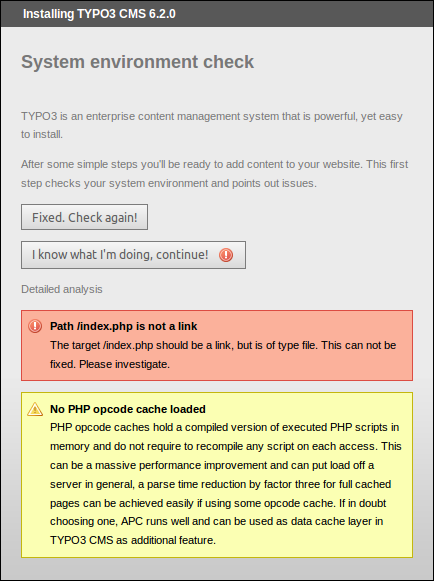
\includegraphics[width=0.8\linewidth]{Images/InstallTool/SystemEnvironmentCheck.png}
			\end{figure}
		\end{column}

	\end{columns}

\end{frame}

% ------------------------------------------------------------------------------
% Re-Development
% ------------------------------------------------------------------------------

\begin{frame}[fragile]
	\frametitle{Install Tool}
	\framesubtitle{Обновление}

	\begin{columns}[T]

		\begin{column}{.5\textwidth}
			\begin{itemize}
				\item \underline{Второй} шаг позволяет ввести сведения о доступе к базе данных
				\item Выбирается тип соединения
					\begin{itemize}
						\item TCP/IP based connection
						\item Socket based connection
					\end{itemize}
				\item Допустимы и альтернативы MySQL
			\end{itemize}
		\end{column}

		\begin{column}{.5\textwidth}
			\begin{figure}\vspace*{-0.4cm}
				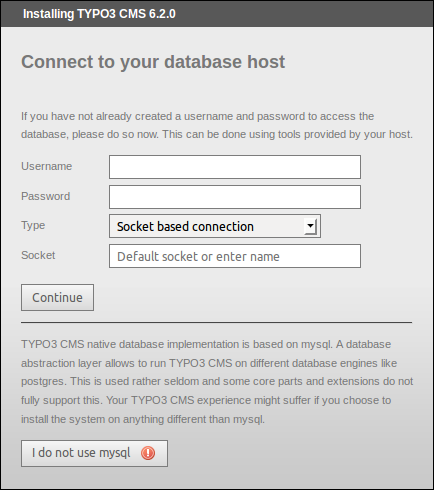
\includegraphics[width=0.8\linewidth]{Images/InstallTool/DatabaseConnectionDetails.png}
			\end{figure}
		\end{column}

	\end{columns}

\end{frame}

% ------------------------------------------------------------------------------
% Re-Development
% ------------------------------------------------------------------------------

\begin{frame}[fragile]
	\frametitle{Install Tool}
	\framesubtitle{Обновление}

	\begin{columns}[T]

		\begin{column}{.5\textwidth}
			\begin{itemize}
				\item \underline{Третий} шаг позволяет выбрать/создать базу данных\newline
					(как и в TYPO3 < 6.2)
				\item \underline{Четвертый} шаг позволяет назначить пароль для пользователя "admin"\newline(который станет и начальным паролем к Install Tool), а также название сайта
			\end{itemize}
		\end{column}

		\begin{column}{.5\textwidth}
			\begin{figure}\vspace*{-0.4cm}
				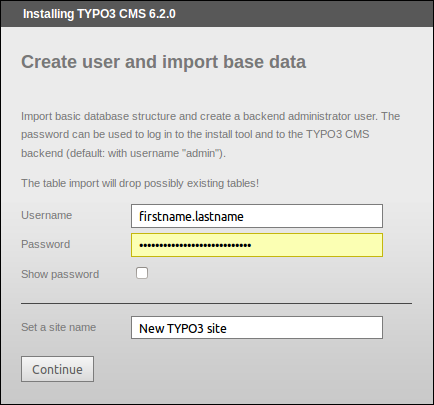
\includegraphics[width=0.8\linewidth]{Images/InstallTool/AdminPasswordAndSiteName.png}
			\end{figure}
		\end{column}

	\end{columns}

\end{frame}

% ------------------------------------------------------------------------------
% Clear all cache
% ------------------------------------------------------------------------------

\begin{frame}[fragile]
	\frametitle{Install Tool}
	\framesubtitle{Очистка кешей}

	\begin{itemize}
		\item Новая функция в разделе "Important actions" позволяет очистить все кеши
		\item Также это срабатывает, если в кеше имеется неверный код PHP\newline
			(что может полностью блокировать TYPO3 CMS)
		\item Обход неработоспособоной TYPO3, с прямым доступом к Install Tool: \texttt{http://example.com/typo3/install}
	\end{itemize}

	\begin{columns}[T]
		\begin{column}{.4\textwidth}
			\begin{figure}\vspace*{-0.4cm}
				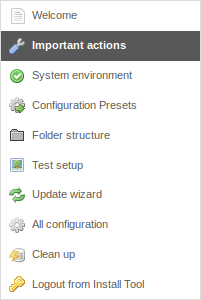
\includegraphics[width=0.7\linewidth]{Images/InstallTool/ImportantActions.png}
			\end{figure}
		\end{column}
		\begin{column}{.6\textwidth}
			\begin{figure}
				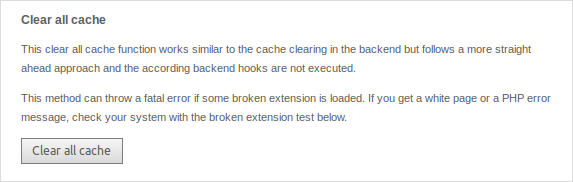
\includegraphics[width=0.9\linewidth]{Images/InstallTool/ClearAllCache.png}
			\end{figure}
		\end{column}
	\end{columns}

\end{frame}

% ------------------------------------------------------------------------------
% Clear all cache
% ------------------------------------------------------------------------------

\begin{frame}[fragile]
	\frametitle{Install Tool}
	\framesubtitle{Очистка кешей}

	Последовательность действий для "Clear all cache" (очистки всех кешей):

	\begin{enumerate}
		\item Удаляется содержимое директории \texttt{typo3temp/Cache}
		\item Очищаются таблицы \texttt{cf\_*}
		\item Загружаются файлы \texttt{ext\_localconf.php} и \texttt{ext\_tables.php}\newline
			из расширений
		\item Выполняется \texttt{flushCaches()}
	\end{enumerate}

\end{frame}

% ------------------------------------------------------------------------------
% Check For Broken Extensions
% ------------------------------------------------------------------------------

\begin{frame}[fragile]
	\frametitle{Install Tool}
	\framesubtitle{Проверка неработоспособных расширений}

	\begin{itemize}
		\item Новая функция в разделе "Important actions" позволяет проверить загрузку расширений без ущерба для работы системы.
		\item Чрезвычайно актуально для обновления от TYPO3 4.5 до 6.2
	\end{itemize}

	\begin{columns}[T]
		\begin{column}{.3\textwidth}
			\begin{figure}\vspace*{-0.4cm}
				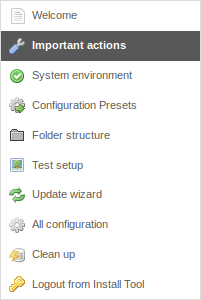
\includegraphics[width=0.7\linewidth]{Images/InstallTool/ImportantActions.png}
			\end{figure}
		\end{column}
		\begin{column}{.7\textwidth}
			\begin{figure}\vspace*{-0.4cm}
				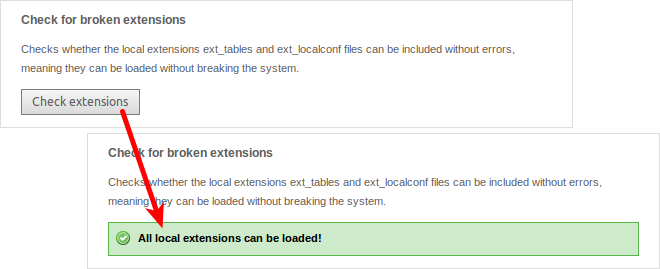
\includegraphics[width=1\linewidth]{Images/InstallTool/CheckForBrokenExtensions.png}
			\end{figure}
		\end{column}
	\end{columns}

\end{frame}

% ------------------------------------------------------------------------------
% Increased Security: Salted Passwords
% ------------------------------------------------------------------------------

\begin{frame}[fragile]
	\frametitle{Install Tool}
	\framesubtitle{Salted Passwords}

	\begin{itemize}
		\item При создании нового пользователя внутреннего интерфейса через Install Tool,
		используется \textbf{salted} пароль\newline
			(требует установленного, загруженного и настроенного EXT:saltedpasswords)
		\item Пароль к Install Tool также \textbf{salted}\newline
			(существующие хеши MD5 автоматически преобразуются при первой авторизации)
	\end{itemize}

	\begin{columns}[T]
		\begin{column}{.3\textwidth}
			\begin{figure}\vspace*{-0.4cm}
				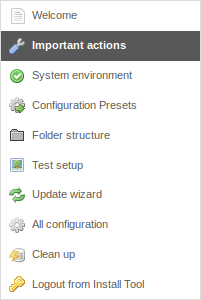
\includegraphics[width=0.7\linewidth]{Images/InstallTool/ImportantActions.png}
			\end{figure}
		\end{column}
		\begin{column}{.7\textwidth}
			\begin{figure}\vspace*{-0.4cm}
				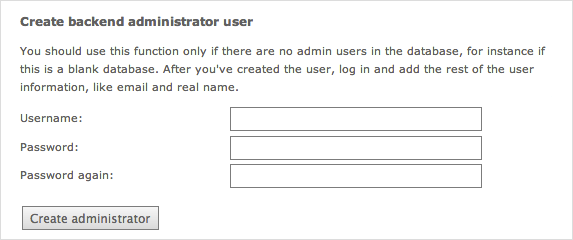
\includegraphics[width=0.9\linewidth]{Images/InstallTool/SaltedPasswords.png}
			\end{figure}
		\end{column}
	\end{columns}

\end{frame}

% ------------------------------------------------------------------------------
% Application Context
% ------------------------------------------------------------------------------

\begin{frame}[fragile]
	\frametitle{Install Tool}
	\framesubtitle{Контекст приложений (1)}

	\begin{itemize}
		\item TYPO3 >= 6.2 учитывает \textbf{Контекст приложений}\newline
			\smaller(известный из TYPO3 Flow)\normalsize
		\item Учитывается набор переменных окружения \texttt{TYPO3\_CONTEXT}\newline
			\smaller(по умолчанию: \texttt{Production}, возможны производные контексты, вроде \texttt{Production/Staging})
			\normalsize

			\begin{lstlisting}
				# File: .htaccess
				# Rules to set Application Context based on hostname:

				RewriteCond %{HTTP_HOST} ^dev\.example\.com$
				RewriteRule (.*) $1 [E=TYPO3_CONTEXT:Development]

				RewriteCond %{HTTP_HOST} ^www\.example\.com$
				RewriteRule (.*) $1 [E=TYPO3_CONTEXT:Production]

				# Sets an environment variable, which is then available to TYPO3 CMS:
				SetEnv TYPO3_CONTEXT Production
			\end{lstlisting}

	\end{itemize}

\end{frame}

% ------------------------------------------------------------------------------
% Application Context
% ------------------------------------------------------------------------------

\begin{frame}[fragile]
	\frametitle{Install Tool}
	\framesubtitle{Набор настроек TYPO3\_CONF\_VAR}

	\begin{columns}[T]
		\begin{column}{.5\textwidth}

			\begin{itemize}
				\item Некоторые \texttt{TYPO3\_CONF\_VAR} параметры можно настроить в Install Tool
				\item Настраиваются такие параметры, как debug output, deprecation log, devIPmask и другие системные
				журналы и их уровни ведения
				\item Встроенные контексты: "Production" и "Development"\newline
					(возможны и пользовательские настройки)
			\end{itemize}

		\end{column}
		\begin{column}{.5\textwidth}

			\begin{figure}\vspace*{-0.4cm}
				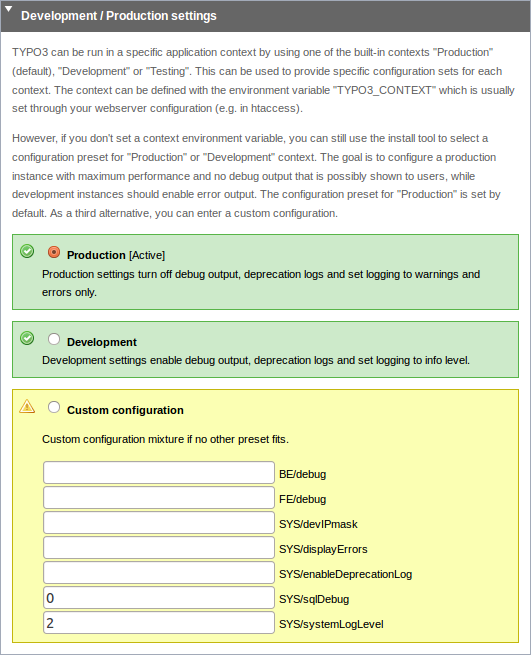
\includegraphics[width=0.8\linewidth]{Images/InstallTool/ApplicationContext.png}
			\end{figure}

		\end{column}
	\end{columns}

\end{frame}

% ------------------------------------------------------------------------------
% Improved Usability
% ------------------------------------------------------------------------------

\begin{frame}[fragile]
	\frametitle{Install Tool}
	\framesubtitle{Улучшенная функциональность}

	\begin{columns}[T]
		\begin{column}{.5\textwidth}

			\begin{itemize}
				\item Исправлено позиционирование меню\newline
				с левой стороны при прокрутке
					\begingroup\color{typo3red}\textbf{(1)}\endgroup
				\item Исправлена позиция кнопки "Write configuration" снизу
					\begingroup\color{typo3red}\textbf{(2)}\endgroup
				\item Отсортированы и сгруппированы элементы в "All Configuration" (разделы раскрываются щелчком по заголовку)
					\begingroup\color{typo3red}\textbf{(3)}\endgroup
			\end{itemize}

		\end{column}
		\begin{column}{.5\textwidth}

			\begin{figure}\vspace*{-0.4cm}
				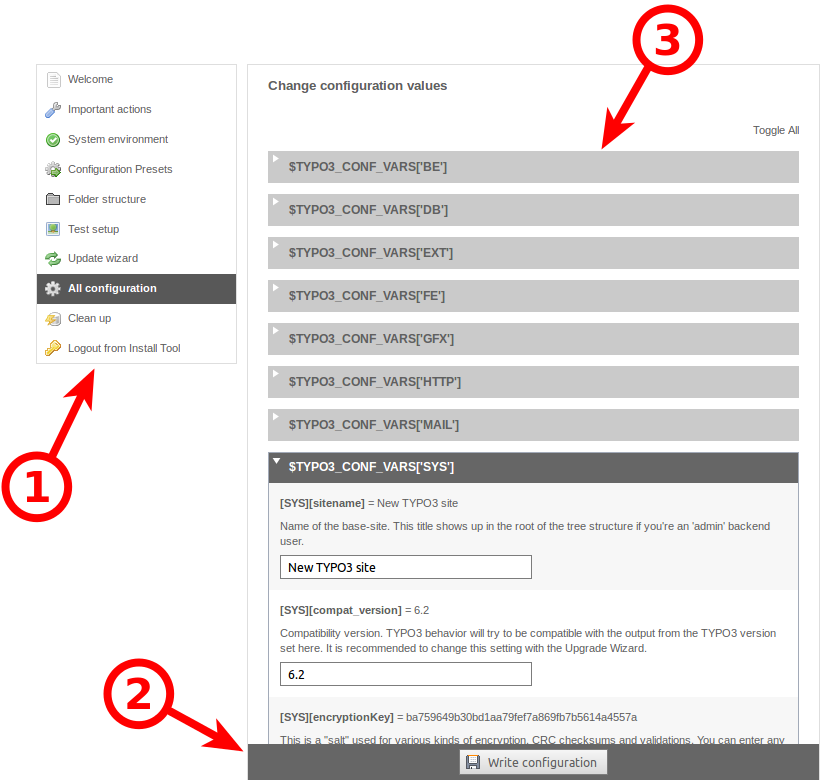
\includegraphics[width=0.8\linewidth]{Images/InstallTool/ImprovedUsability.png}
			\end{figure}

		\end{column}
	\end{columns}

\end{frame}

% ------------------------------------------------------------------------------
% Human-Friendly Error Codes
% ------------------------------------------------------------------------------

\begin{frame}[fragile]
	\frametitle{Install Tool}
	\framesubtitle{Понятные коды ошибок}

	\begin{itemize}
		\item Для следующих параметров возможно использовать значимые ключи:\newline
			(TYPO3 < 6.2: только числовые коды)
	\end{itemize}

	\begin{columns}[T]
		\begin{column}{.4\textwidth}
			\advance\leftskip+0.8cm

			\smaller
				\texttt{[SYS][errorHandlerErrors]}\newline
				\texttt{[SYS][exceptionalErrors]}\newline
				\texttt{[SYS][syslogErrorReporting]}\newline
				\texttt{[SYS][belogErrorReporting]}\newline
			\normalsize

		\end{column}
		\begin{column}{.6\textwidth}

			\begin{figure}\vspace*{-0.4cm}
				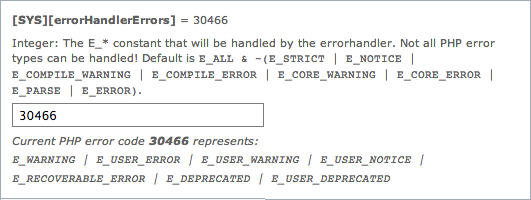
\includegraphics[width=0.9\linewidth]{Images/InstallTool/HumanFriendlyErrorCodes.png}
			\end{figure}

		\end{column}
	\end{columns}

	\vspace{0.2cm}

	\begin{itemize}
		\item Проектор (ViewHelper) Extbase \textbf{format.phpErrorCode} заботиться о преобразовании в коды ошибок PHP
	\end{itemize}

\end{frame}

% ------------------------------------------------------------------------------
% Errors In Folder Structure
% ------------------------------------------------------------------------------

\begin{frame}[fragile]
	\frametitle{Install Tool}
	\framesubtitle{Ошибки в структуре папок}

	\begin{itemize}
		\item Ошибки  "Folder Structure" (структуре папок) представлены как значок (номер в круге)
	\end{itemize}

	\begin{figure}
		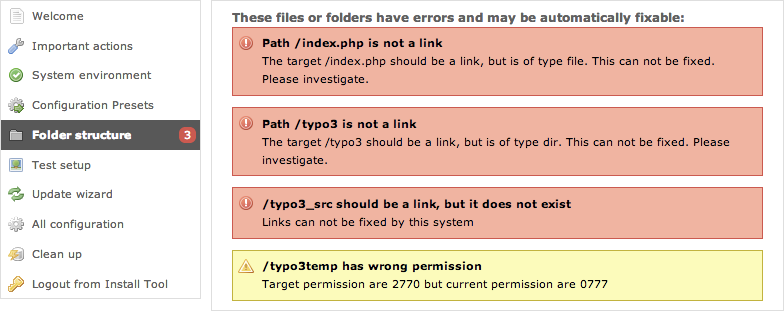
\includegraphics[width=0.95\linewidth]{Images/InstallTool/ErrorsInFolderStructure.png}
	\end{figure}

\end{frame}

% ------------------------------------------------------------------------------
% Core Updates
% ------------------------------------------------------------------------------

\begin{frame}[fragile]
	\frametitle{Install Tool}
	\framesubtitle{Обновления ядра}

	\begin{itemize}
		\item Обновления ядра TYPO3 на следующую промежуточную версию щелчком по кнопке
		\item Переменная окружения \texttt{TYPO3\_DISABLE\_CORE\_UPDATER=1} отключит эту возможность
	\end{itemize}

	\begin{figure}
		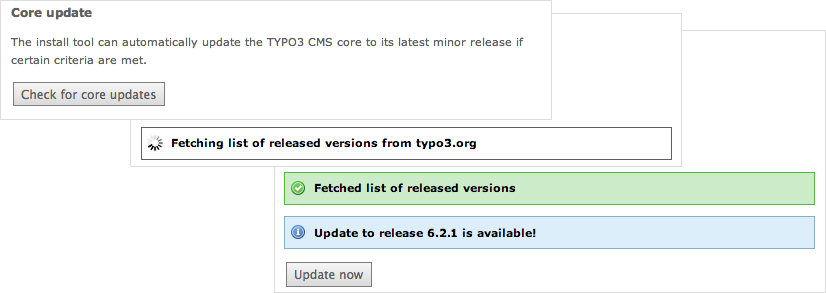
\includegraphics[width=0.95\linewidth]{Images/InstallTool/CoreUpdate.png}
	\end{figure}

\end{frame}

% ------------------------------------------------------------------------------
% Miscellaneous
% ------------------------------------------------------------------------------

\begin{frame}[fragile]
	\frametitle{Install Tool}
	\framesubtitle{Доработки}

	\begin{itemize}
		\item Все формы CSRF - защищенные (\textit{cross-site request forgery - межсайтовая подделка запросов})
		\item Install Tool использует упрощенный Fluid Standalone View
		\item Загружаются лишь важнейшие функции TYPO3\newline
			(поврежденные \texttt{ext\_localconf.php} или \texttt{ext\_tables.php} в расширениях более не смогут повлиять на
			работу Install Tool)
		\item Новая отправная точка:	\tabto{3.2cm} \texttt{typo3/sysext/install/Start/Install.php}\newline
			До:					\tabto{3.2cm} \texttt{typo3/install/index.php}\newline
									\tabto{3.2cm} (существует перенаправление от старого к новому URL)
		\item Отключение кеша гарантирует работу Install Tool даже при ошибках в коде PHP в кеше
	\end{itemize}

\end{frame}

% ------------------------------------------------------------------------------
% Miscellaneous
% ------------------------------------------------------------------------------

\begin{frame}[fragile]
	\frametitle{Install Tool}
	\framesubtitle{Доработки}

	\begin{itemize}
		\item Убедитесь, что параметр PHP \texttt{xdebug.max\_nesting\_level} имеет значение 250 или выше (значение "100" по умолчанию, может вызвать проблемы)
		\item "Relaxed permission check" - ослабление в проверке разрешений:

			\small
				Если корневая web папка сервера не имеет правильных разрешений (например, "2770"),
				и это нельзя исправить, например, папка не принадлежит системному пользователю,
				выполняющему Install Tool, установка прерывается на первом шаге.
				Параметр "targetPermissionRelaxed" понижает требования к безопасности, и позволяет
				продолжить установку, пока не будут созданы необходимые папки.
			\normalsize

	\end{itemize}

\end{frame}

% ------------------------------------------------------------------------------
% Miscellaneous
% ------------------------------------------------------------------------------

\begin{frame}[fragile]
	\frametitle{Install Tool}
	\framesubtitle{Доработки}

	\begin{itemize}
		\item Удаленные из Install Tool параметры (ключи) \newline
			(а, значит, также и из файла \texttt{LocalConfiguration.php}):
	\end{itemize}

	\begin{columns}[T]
		\begin{column}{.5\textwidth}
			\advance\leftskip+0.8cm
			\smaller
				\texttt{BE/loginLabels}\newline
				\texttt{BE/loginNews}\newline
				\texttt{BE/useOnContextMenuHandler}\newline
				\texttt{EXT/em\_mirrorListURL}\newline
				\texttt{EXT/em\_wsdlURL}\newline
				\texttt{EXT/extList}\newline
				\texttt{EXT/extList\_FE}\newline
				\texttt{EXT/noEdit}\newline
			\normalsize
		\end{column}
		\begin{column}{.5\textwidth}
			\smaller
				\texttt{FE/defaultTypoScript\_editorcfg}\newline
				\texttt{FE/simulateStaticDocuments}\newline
				\texttt{GFX/noIconProc}\newline
				\texttt{GFX/TTFLocaleConv}\newline
				\texttt{SYS/additionalAllowedClassPrefixes}\newline
				\texttt{SYS/caching/cacheBackends}\newline
				\texttt{SYS/caching/cacheFrontends}\newline
				\texttt{SYS/extCache}\newline
				\texttt{SYS/T3instID}\newline
			\normalsize
		\end{column}

	\end{columns}

\end{frame}

% ------------------------------------------------------------------------------

